% id: 0502
% book: RPM 중3-2 수학 · 04 원주각
% section: 중단원 마무리하기
% figure: crop:fig-0502.png
% answer: ⑤
% answer_source: 답지
% variant_level: 0 (원본 전사)
% 이 파일은 build.mjs 가 items.json 에서 만든다. 고칠 때는 items.json 을 고친다.
\noindent\begin{minipage}[t]{0.58\linewidth}\vspace{0pt}\raggedright 오른쪽 그림에서 $\arc{AB}:\arc{BC}:\arc{CA}=1:2:3$일 때, 다음 중 옳지 \underline{않은} 것은?\end{minipage}\hfill\begin{minipage}[t]{0.4\linewidth}\vspace{0pt}\centering \setlength{\dmfigw}{61.8pt}\ifdim\dmfigw>\linewidth\setlength{\dmfigw}{\linewidth}\fi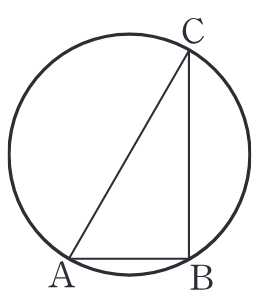
\includegraphics[width=\dmfigw]{figures/fig-0502.png}\end{minipage}\par
\par\medskip\par\noindent\hangindent=1.4em\hangafter=1 {\small ①}\ $\angle\pt{CAB}=60^\circ$\par\noindent\hangindent=1.4em\hangafter=1 {\small ②}\ $\angle\pt{ABC}=90^\circ$\par\noindent\hangindent=1.4em\hangafter=1 {\small ③}\ $\angle\pt{ACB}=30^\circ$\par\noindent\hangindent=1.4em\hangafter=1 {\small ④}\ $\triangle\pt{ABC}$는 직각삼각형이다.\par\noindent\hangindent=1.4em\hangafter=1 {\small ⑤}\ $\arc{BC}=6\pi\mkern3mu \mathrm{cm}$이면 $\arc{CA}=8\pi\mkern3mu \mathrm{cm}$이다.\par\medskip
